% Options for packages loaded elsewhere
\PassOptionsToPackage{unicode}{hyperref}
\PassOptionsToPackage{hyphens}{url}
\PassOptionsToPackage{dvipsnames,svgnames,x11names}{xcolor}
%
\documentclass[
  letterpaper,
  DIV=11,
  numbers=noendperiod]{scrartcl}

\usepackage{amsmath,amssymb}
\usepackage{iftex}
\ifPDFTeX
  \usepackage[T1]{fontenc}
  \usepackage[utf8]{inputenc}
  \usepackage{textcomp} % provide euro and other symbols
\else % if luatex or xetex
  \usepackage{unicode-math}
  \defaultfontfeatures{Scale=MatchLowercase}
  \defaultfontfeatures[\rmfamily]{Ligatures=TeX,Scale=1}
\fi
\usepackage{lmodern}
\ifPDFTeX\else  
    % xetex/luatex font selection
\fi
% Use upquote if available, for straight quotes in verbatim environments
\IfFileExists{upquote.sty}{\usepackage{upquote}}{}
\IfFileExists{microtype.sty}{% use microtype if available
  \usepackage[]{microtype}
  \UseMicrotypeSet[protrusion]{basicmath} % disable protrusion for tt fonts
}{}
\makeatletter
\@ifundefined{KOMAClassName}{% if non-KOMA class
  \IfFileExists{parskip.sty}{%
    \usepackage{parskip}
  }{% else
    \setlength{\parindent}{0pt}
    \setlength{\parskip}{6pt plus 2pt minus 1pt}}
}{% if KOMA class
  \KOMAoptions{parskip=half}}
\makeatother
\usepackage{xcolor}
\setlength{\emergencystretch}{3em} % prevent overfull lines
\setcounter{secnumdepth}{5}
% Make \paragraph and \subparagraph free-standing
\ifx\paragraph\undefined\else
  \let\oldparagraph\paragraph
  \renewcommand{\paragraph}[1]{\oldparagraph{#1}\mbox{}}
\fi
\ifx\subparagraph\undefined\else
  \let\oldsubparagraph\subparagraph
  \renewcommand{\subparagraph}[1]{\oldsubparagraph{#1}\mbox{}}
\fi

\usepackage{color}
\usepackage{fancyvrb}
\newcommand{\VerbBar}{|}
\newcommand{\VERB}{\Verb[commandchars=\\\{\}]}
\DefineVerbatimEnvironment{Highlighting}{Verbatim}{commandchars=\\\{\}}
% Add ',fontsize=\small' for more characters per line
\usepackage{framed}
\definecolor{shadecolor}{RGB}{241,243,245}
\newenvironment{Shaded}{\begin{snugshade}}{\end{snugshade}}
\newcommand{\AlertTok}[1]{\textcolor[rgb]{0.68,0.00,0.00}{#1}}
\newcommand{\AnnotationTok}[1]{\textcolor[rgb]{0.37,0.37,0.37}{#1}}
\newcommand{\AttributeTok}[1]{\textcolor[rgb]{0.40,0.45,0.13}{#1}}
\newcommand{\BaseNTok}[1]{\textcolor[rgb]{0.68,0.00,0.00}{#1}}
\newcommand{\BuiltInTok}[1]{\textcolor[rgb]{0.00,0.23,0.31}{#1}}
\newcommand{\CharTok}[1]{\textcolor[rgb]{0.13,0.47,0.30}{#1}}
\newcommand{\CommentTok}[1]{\textcolor[rgb]{0.37,0.37,0.37}{#1}}
\newcommand{\CommentVarTok}[1]{\textcolor[rgb]{0.37,0.37,0.37}{\textit{#1}}}
\newcommand{\ConstantTok}[1]{\textcolor[rgb]{0.56,0.35,0.01}{#1}}
\newcommand{\ControlFlowTok}[1]{\textcolor[rgb]{0.00,0.23,0.31}{#1}}
\newcommand{\DataTypeTok}[1]{\textcolor[rgb]{0.68,0.00,0.00}{#1}}
\newcommand{\DecValTok}[1]{\textcolor[rgb]{0.68,0.00,0.00}{#1}}
\newcommand{\DocumentationTok}[1]{\textcolor[rgb]{0.37,0.37,0.37}{\textit{#1}}}
\newcommand{\ErrorTok}[1]{\textcolor[rgb]{0.68,0.00,0.00}{#1}}
\newcommand{\ExtensionTok}[1]{\textcolor[rgb]{0.00,0.23,0.31}{#1}}
\newcommand{\FloatTok}[1]{\textcolor[rgb]{0.68,0.00,0.00}{#1}}
\newcommand{\FunctionTok}[1]{\textcolor[rgb]{0.28,0.35,0.67}{#1}}
\newcommand{\ImportTok}[1]{\textcolor[rgb]{0.00,0.46,0.62}{#1}}
\newcommand{\InformationTok}[1]{\textcolor[rgb]{0.37,0.37,0.37}{#1}}
\newcommand{\KeywordTok}[1]{\textcolor[rgb]{0.00,0.23,0.31}{#1}}
\newcommand{\NormalTok}[1]{\textcolor[rgb]{0.00,0.23,0.31}{#1}}
\newcommand{\OperatorTok}[1]{\textcolor[rgb]{0.37,0.37,0.37}{#1}}
\newcommand{\OtherTok}[1]{\textcolor[rgb]{0.00,0.23,0.31}{#1}}
\newcommand{\PreprocessorTok}[1]{\textcolor[rgb]{0.68,0.00,0.00}{#1}}
\newcommand{\RegionMarkerTok}[1]{\textcolor[rgb]{0.00,0.23,0.31}{#1}}
\newcommand{\SpecialCharTok}[1]{\textcolor[rgb]{0.37,0.37,0.37}{#1}}
\newcommand{\SpecialStringTok}[1]{\textcolor[rgb]{0.13,0.47,0.30}{#1}}
\newcommand{\StringTok}[1]{\textcolor[rgb]{0.13,0.47,0.30}{#1}}
\newcommand{\VariableTok}[1]{\textcolor[rgb]{0.07,0.07,0.07}{#1}}
\newcommand{\VerbatimStringTok}[1]{\textcolor[rgb]{0.13,0.47,0.30}{#1}}
\newcommand{\WarningTok}[1]{\textcolor[rgb]{0.37,0.37,0.37}{\textit{#1}}}

\providecommand{\tightlist}{%
  \setlength{\itemsep}{0pt}\setlength{\parskip}{0pt}}\usepackage{longtable,booktabs,array}
\usepackage{calc} % for calculating minipage widths
% Correct order of tables after \paragraph or \subparagraph
\usepackage{etoolbox}
\makeatletter
\patchcmd\longtable{\par}{\if@noskipsec\mbox{}\fi\par}{}{}
\makeatother
% Allow footnotes in longtable head/foot
\IfFileExists{footnotehyper.sty}{\usepackage{footnotehyper}}{\usepackage{footnote}}
\makesavenoteenv{longtable}
\usepackage{graphicx}
\makeatletter
\def\maxwidth{\ifdim\Gin@nat@width>\linewidth\linewidth\else\Gin@nat@width\fi}
\def\maxheight{\ifdim\Gin@nat@height>\textheight\textheight\else\Gin@nat@height\fi}
\makeatother
% Scale images if necessary, so that they will not overflow the page
% margins by default, and it is still possible to overwrite the defaults
% using explicit options in \includegraphics[width, height, ...]{}
\setkeys{Gin}{width=\maxwidth,height=\maxheight,keepaspectratio}
% Set default figure placement to htbp
\makeatletter
\def\fps@figure{htbp}
\makeatother

\usepackage{booktabs}
\usepackage{caption}
\usepackage{longtable}
\usepackage{colortbl}
\usepackage{array}
\KOMAoption{captions}{tableheading}
\makeatletter
\@ifpackageloaded{tcolorbox}{}{\usepackage[skins,breakable]{tcolorbox}}
\@ifpackageloaded{fontawesome5}{}{\usepackage{fontawesome5}}
\definecolor{quarto-callout-color}{HTML}{909090}
\definecolor{quarto-callout-note-color}{HTML}{0758E5}
\definecolor{quarto-callout-important-color}{HTML}{CC1914}
\definecolor{quarto-callout-warning-color}{HTML}{EB9113}
\definecolor{quarto-callout-tip-color}{HTML}{00A047}
\definecolor{quarto-callout-caution-color}{HTML}{FC5300}
\definecolor{quarto-callout-color-frame}{HTML}{acacac}
\definecolor{quarto-callout-note-color-frame}{HTML}{4582ec}
\definecolor{quarto-callout-important-color-frame}{HTML}{d9534f}
\definecolor{quarto-callout-warning-color-frame}{HTML}{f0ad4e}
\definecolor{quarto-callout-tip-color-frame}{HTML}{02b875}
\definecolor{quarto-callout-caution-color-frame}{HTML}{fd7e14}
\makeatother
\makeatletter
\makeatother
\makeatletter
\makeatother
\makeatletter
\@ifpackageloaded{caption}{}{\usepackage{caption}}
\AtBeginDocument{%
\ifdefined\contentsname
  \renewcommand*\contentsname{Table of contents}
\else
  \newcommand\contentsname{Table of contents}
\fi
\ifdefined\listfigurename
  \renewcommand*\listfigurename{List of Figures}
\else
  \newcommand\listfigurename{List of Figures}
\fi
\ifdefined\listtablename
  \renewcommand*\listtablename{List of Tables}
\else
  \newcommand\listtablename{List of Tables}
\fi
\ifdefined\figurename
  \renewcommand*\figurename{Figure}
\else
  \newcommand\figurename{Figure}
\fi
\ifdefined\tablename
  \renewcommand*\tablename{Table}
\else
  \newcommand\tablename{Table}
\fi
}
\@ifpackageloaded{float}{}{\usepackage{float}}
\floatstyle{ruled}
\@ifundefined{c@chapter}{\newfloat{codelisting}{h}{lop}}{\newfloat{codelisting}{h}{lop}[chapter]}
\floatname{codelisting}{Listing}
\newcommand*\listoflistings{\listof{codelisting}{List of Listings}}
\makeatother
\makeatletter
\@ifpackageloaded{caption}{}{\usepackage{caption}}
\@ifpackageloaded{subcaption}{}{\usepackage{subcaption}}
\makeatother
\makeatletter
\@ifpackageloaded{tcolorbox}{}{\usepackage[skins,breakable]{tcolorbox}}
\makeatother
\makeatletter
\@ifundefined{shadecolor}{\definecolor{shadecolor}{rgb}{.97, .97, .97}}
\makeatother
\makeatletter
\makeatother
\makeatletter
\makeatother
\ifLuaTeX
  \usepackage{selnolig}  % disable illegal ligatures
\fi
\IfFileExists{bookmark.sty}{\usepackage{bookmark}}{\usepackage{hyperref}}
\IfFileExists{xurl.sty}{\usepackage{xurl}}{} % add URL line breaks if available
\urlstyle{same} % disable monospaced font for URLs
\hypersetup{
  pdftitle={Week 5: Introduction to Quarto},
  colorlinks=true,
  linkcolor={blue},
  filecolor={Maroon},
  citecolor={Blue},
  urlcolor={Blue},
  pdfcreator={LaTeX via pandoc}}

\title{Week 5: Introduction to Quarto}
\author{}
\date{}

\begin{document}
\maketitle
\ifdefined\Shaded\renewenvironment{Shaded}{\begin{tcolorbox}[sharp corners, interior hidden, boxrule=0pt, breakable, borderline west={3pt}{0pt}{shadecolor}, frame hidden, enhanced]}{\end{tcolorbox}}\fi

\renewcommand*\contentsname{Contents}
{
\hypersetup{linkcolor=}
\setcounter{tocdepth}{3}
\tableofcontents
}
\hypertarget{introduction}{%
\section{Introduction}\label{introduction}}

This week we will take what we have learned in previous weeks and
produce a report using Quarto . Quarto is a multi-language system that
allows reports and presentation to be created within R, thus allowing
for R code and output to be easily embedded within a report, a
presentation or even a Blog!. Hence, all of the R code and plots
obtained from an analysis are contained within a single file.

Under Week 5 on Moodle there is an Example Report produced using Quarto
relating to fitting a regression model using one numerical explanatory
variable that was done in Week 4. The corresponding Quarto \texttt{.qmd}
file can also be downloaded and opened in R to see how the document was
produced (press the \texttt{Render} button to create the HTML/PDF
version). It is advised to have this document open within RStudio while
working through the remaining sections in order to see examples put into
practice.

The following sections will take you through the different steps
required to produce the Example Report on Moodle. For creating a new
Quarto file from scratch see Section 1.1, otherwise move onto Section 2.

\hypertarget{creating-a-new-quarto-document-from-scratch}{%
\subsection{Creating a new Quarto document from
scratch}\label{creating-a-new-quarto-document-from-scratch}}

If you want to create a new R Markdown document from scratch within
RStudio you can go to:

\texttt{File\ -\textgreater{}\ New\ File\ -\textgreater{}\ Quarto\ \ Document...}

This will open the following window within RStudio:

\begin{figure}

{\centering 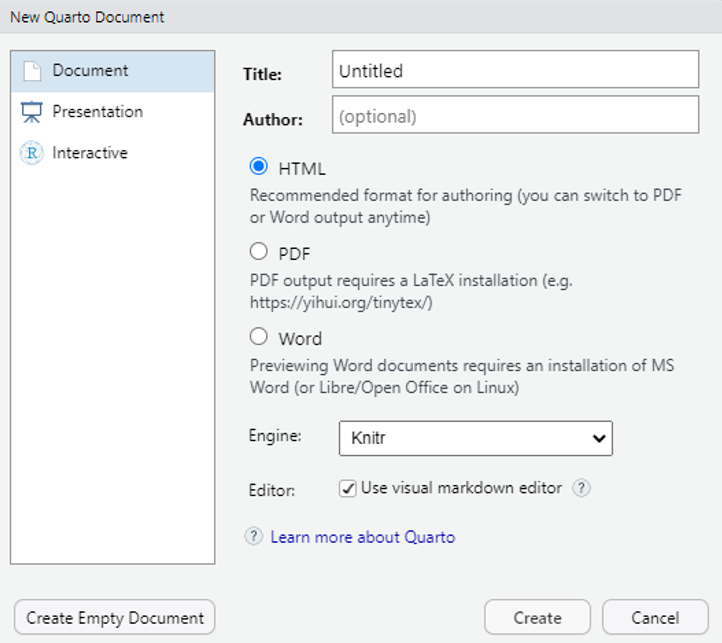
\includegraphics[width=5.20833in,height=\textheight]{images/quarto1.png}

}

\end{figure}

\begin{tcolorbox}[enhanced jigsaw, colback=white, toprule=.15mm, arc=.35mm, colbacktitle=quarto-callout-important-color!10!white, titlerule=0mm, colframe=quarto-callout-important-color-frame, title=\textcolor{quarto-callout-important-color}{\faExclamation}\hspace{0.5em}{Important}, bottomtitle=1mm, toptitle=1mm, coltitle=black, rightrule=.15mm, opacityback=0, bottomrule=.15mm, breakable, leftrule=.75mm, left=2mm, opacitybacktitle=0.6]

Before creating your first Quarto document, be sure that you have the
latest RStudio
\href{https://posit.co/download/rstudio-desktop/}{version} installed.

\end{tcolorbox}

From here select \textbf{Document} and the \textbf{Default Output
Format} as \textbf{PDF} or \textbf{HTML}. Give your document a title and
select OK. This will open within RStudio an empty \texttt{.qmd} file.

\begin{tcolorbox}[enhanced jigsaw, colback=white, toprule=.15mm, arc=.35mm, colbacktitle=quarto-callout-note-color!10!white, titlerule=0mm, colframe=quarto-callout-note-color-frame, title=\textcolor{quarto-callout-note-color}{\faInfo}\hspace{0.5em}{Note}, bottomtitle=1mm, toptitle=1mm, coltitle=black, rightrule=.15mm, opacityback=0, bottomrule=.15mm, breakable, leftrule=.75mm, left=2mm, opacitybacktitle=0.6]

You can download this
\href{https://quarto.org/docs/get-started/hello/rstudio/_hello.qmd}{template}
containing simple instructions on how to do some basic stuff using
Quarto . To see what the HTML/PDF of the template document looks like
click on the

\includegraphics[width=0.16667in,height=0.13542in]{images/rstudio-render-button.png}
\texttt{Render} button at the top of the document window.

\end{tcolorbox}

\hypertarget{title}{%
\section{Title}\label{title}}

The title of the document can be found at the top of the \texttt{.qmd}
file within its preamble, which is shown below. When titling your
document, ensure the title is within inverted commas.

\begin{verbatim}
---
title: "Example Report"
---
\end{verbatim}

A Quarto document can be edited in the two modes of the RStudio editor:
visual (on the left) and source (on the right). The visual mode offers a
more friendly interface for editing you document (it includes a toolbar
for quick edit options), while the source mode allows you to see and
edit the underlying R markdown text code.

\begin{figure}

{\centering 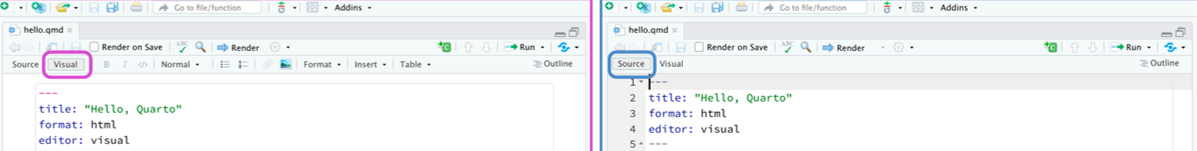
\includegraphics[width=7.94792in,height=\textheight]{images/quarto2.png}

}

\end{figure}

You can switch between these two modes at anytime. Will now cover
different aspects of building a Quarto document and provide the
instructions on how to do this using either the visual editor or the
source mode.

\hypertarget{sections}{%
\section{Sections}\label{sections}}

Under the \texttt{source} mode, sections within a Quarto document are
created using \texttt{\#}. For example, \texttt{\#\ Introduction} will
create a section titled \textbf{Introduction}. Alternatively, if you use
the \texttt{visual} mode, you can include a new section by selecting a
proper heading under the block-format display of the toolbar as follows:

\begin{figure}

{\centering 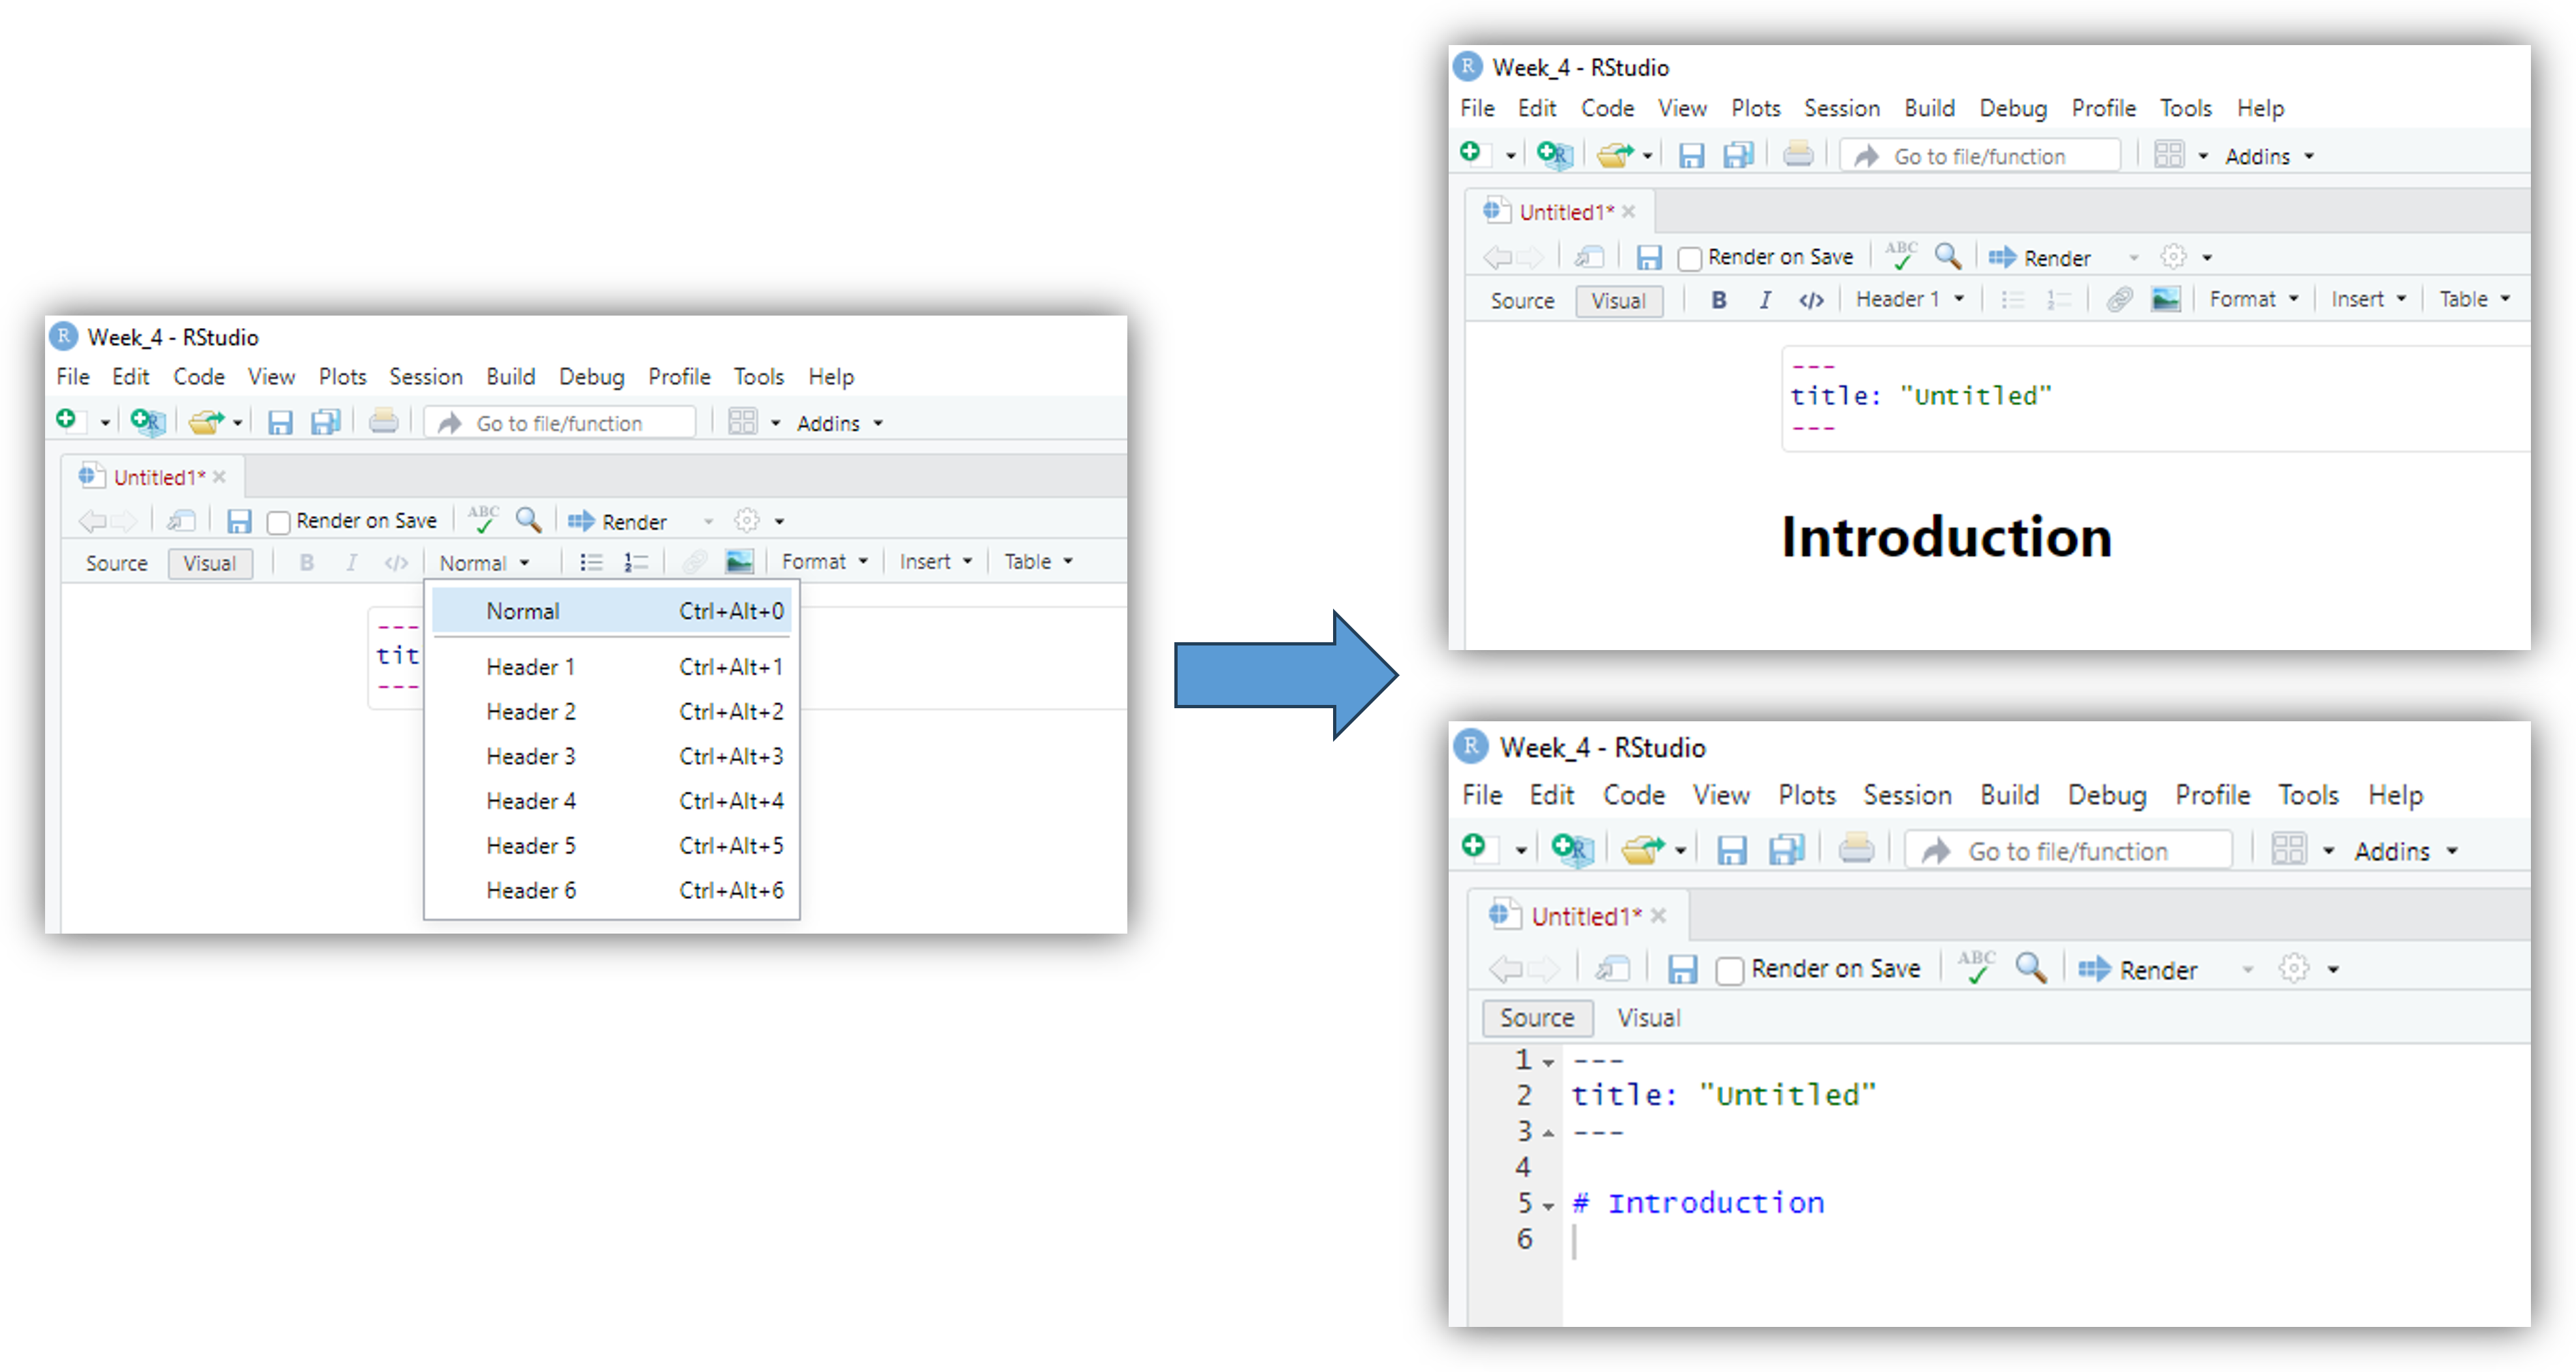
\includegraphics[width=7.64583in,height=\textheight]{images/quarto3.png}

}

\end{figure}

If you want section to be numbered you can set
\texttt{number\_sections:\ true} within the preamble of the document:

\begin{verbatim}
---
title: "My title"
number-sections: true
---
\end{verbatim}

Each section can be assigned labels so that they can be referred to
within the text. To reference a section, add
a~\texttt{\#sec-}~identifier to any heading. For example, to give our
\textbf{Introduction} section a label we simply add the label
\texttt{\{\#sec-intro\}} to the section title as follows:

\begin{verbatim}
# Introduction {#sec-intro}
\end{verbatim}

where \texttt{sec-intro} is the name chosen for this particular section.
For the \texttt{visual} model you can click on the edit attributes
settings

\includegraphics[width=0.17708in,height=\textheight]{images/threedots.png}
(right hand side of the section heading) and write the label you want on
the ID box of the pop-up window:

\begin{figure}

{\centering 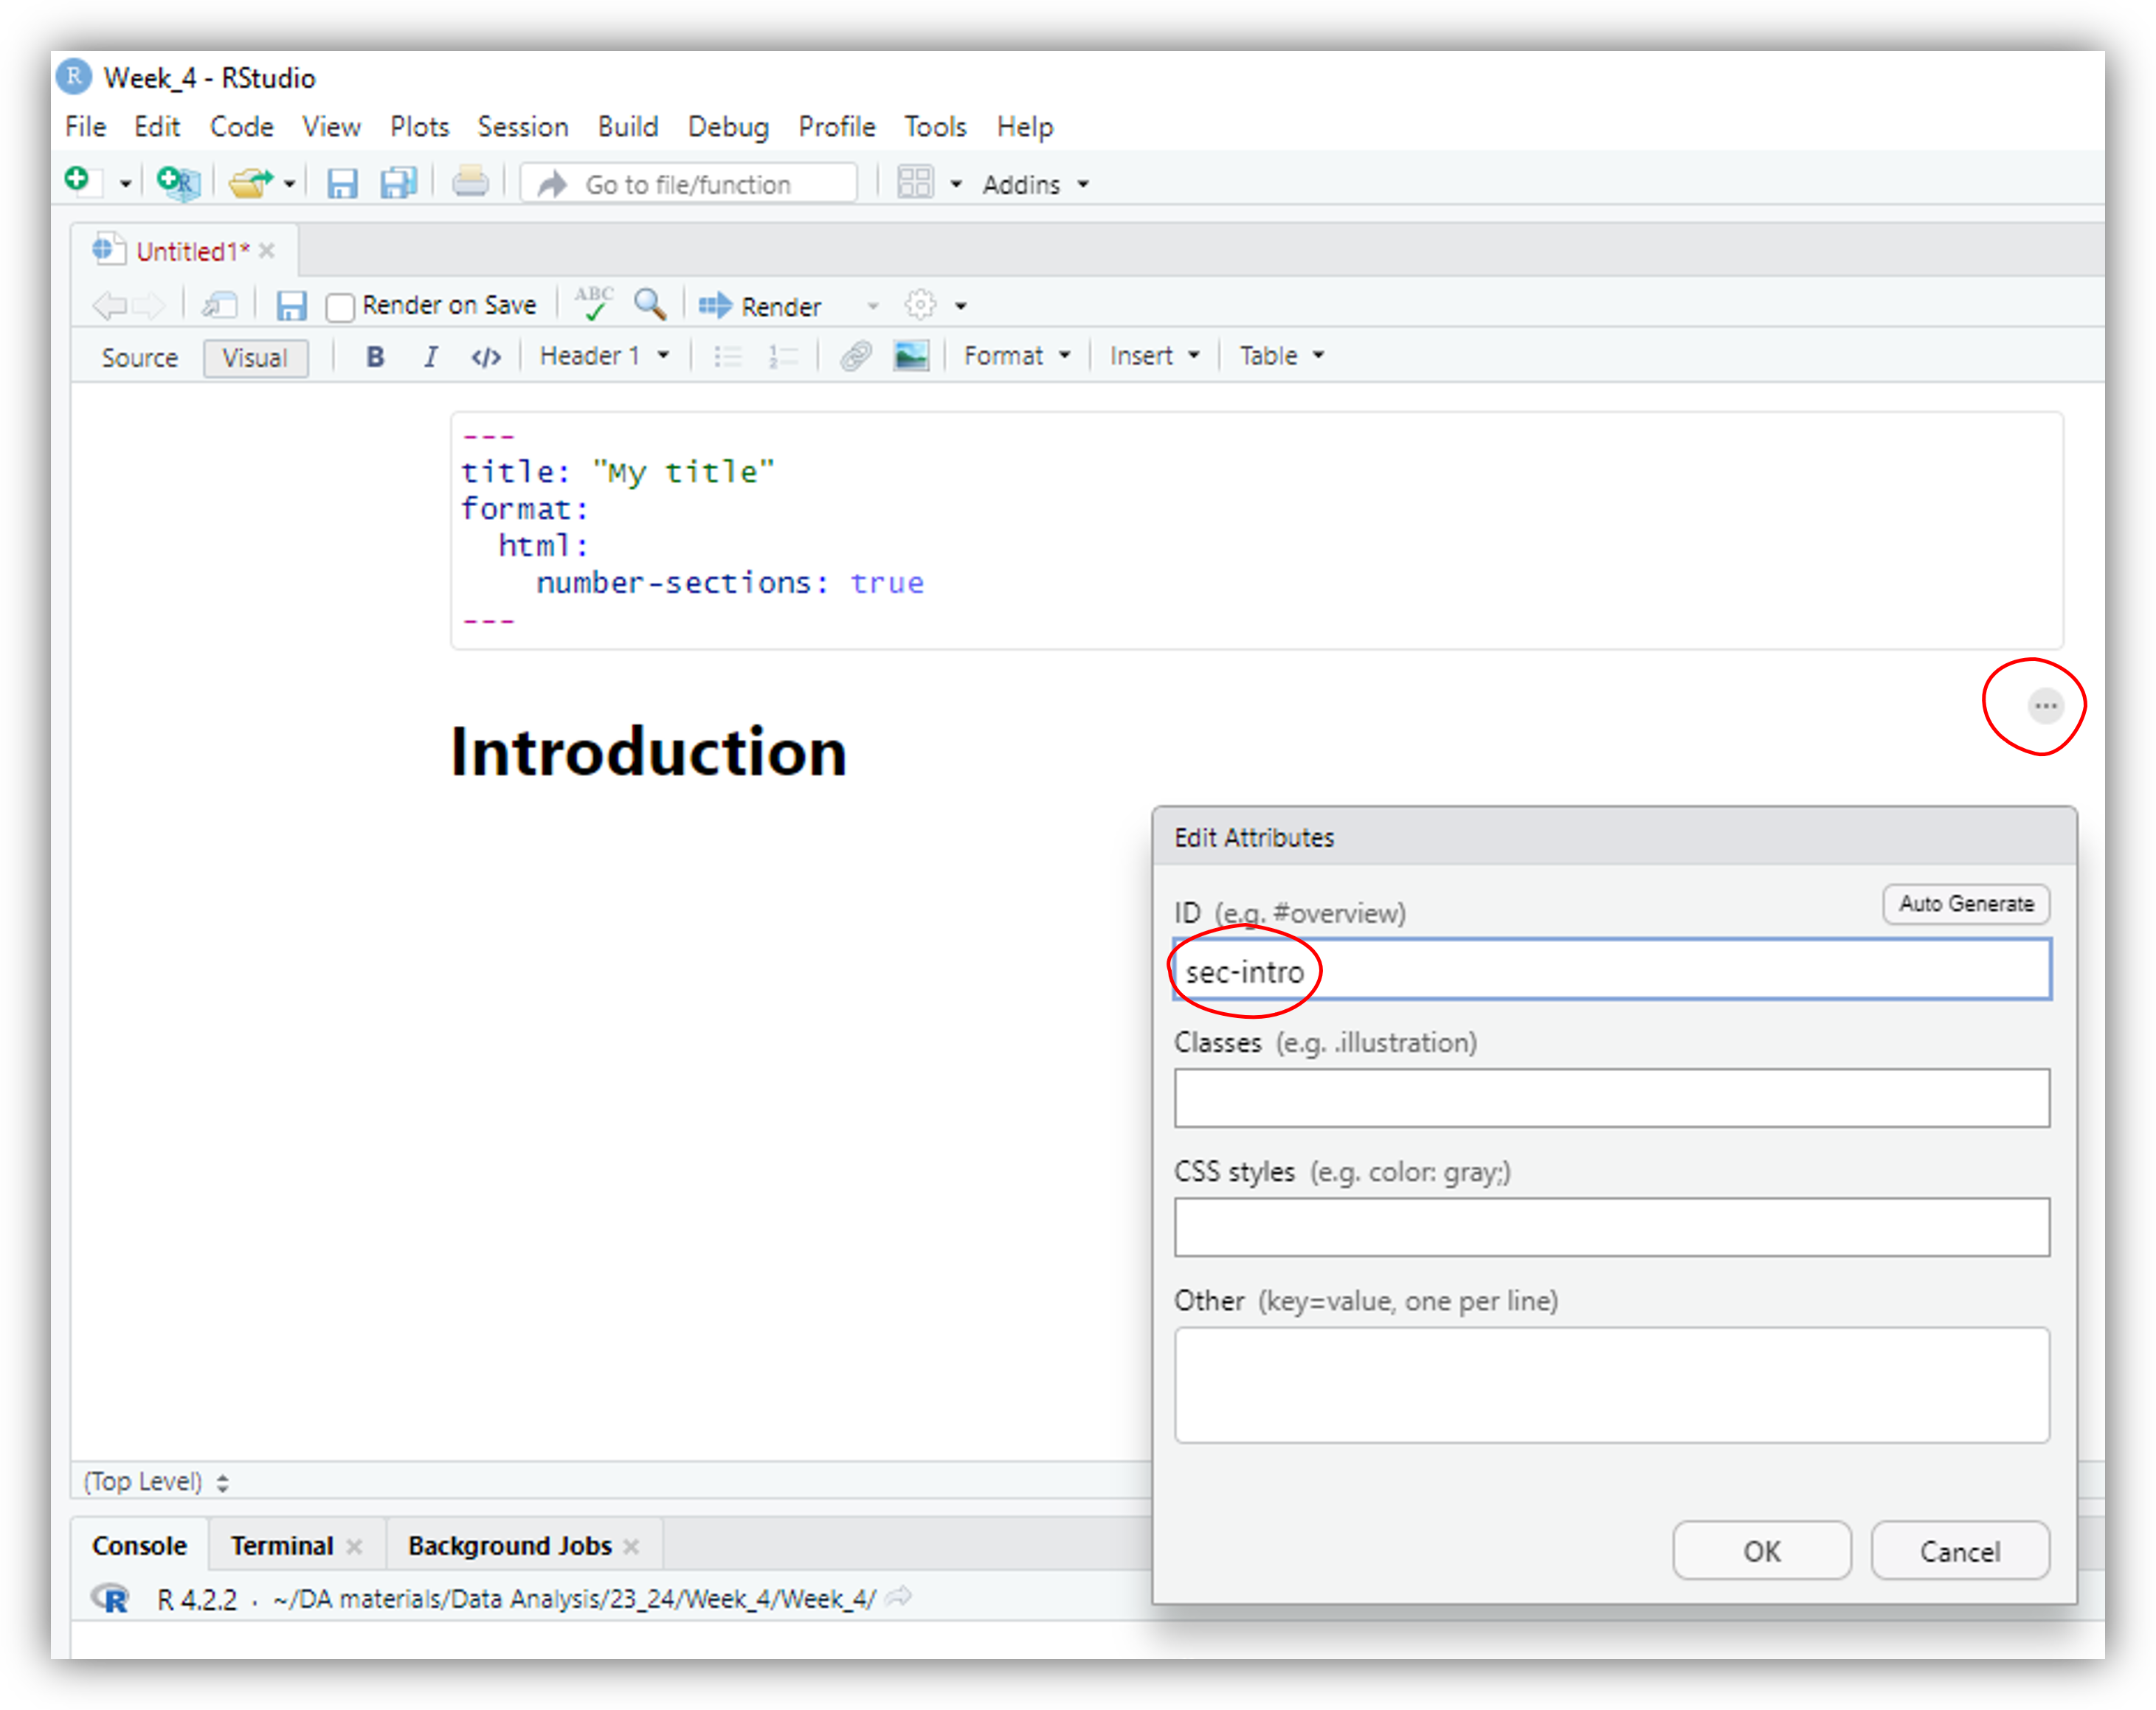
\includegraphics{images/quarto4.png}

}

\end{figure}

\begin{tcolorbox}[enhanced jigsaw, colback=white, toprule=.15mm, arc=.35mm, colbacktitle=quarto-callout-important-color!10!white, titlerule=0mm, colframe=quarto-callout-important-color-frame, title=\textcolor{quarto-callout-important-color}{\faExclamation}\hspace{0.5em}{Important}, bottomtitle=1mm, toptitle=1mm, coltitle=black, rightrule=.15mm, opacityback=0, bottomrule=.15mm, breakable, leftrule=.75mm, left=2mm, opacitybacktitle=0.6]

It is a good idea to label your sections appropriately so that it is
easy to refer to them later. Note that it is important to add the
\texttt{sec-} prefix in order for cross-referencing to work properly.

\end{tcolorbox}

The section can now be referred to within the text of the document using
the \texttt{@}sec- command. That is

\begin{verbatim}
Section @sec-intro ...
\end{verbatim}

will produce

\begin{verbatim}
Section 1 ...
\end{verbatim}

where the 1 is a clickable hyperlink that will take you to the beginning
of that section within the document. If you are using the
\texttt{visual} mode, you can easily include cross-references by
clicking on \texttt{Insert▾➠\ Cross\ Reference}

Note that for section labels to appear on the references list, you must
save your document first (click on \texttt{File\ ➠\ Save\ as…} and save
your document with a proper name). Then all the labels (i.e., labels of
sections, figures, equations, etc.) will appear on the Insert Cross
Reference pop up window. Then simply click on \texttt{Insert▾} to add
the selected reference to your document.

\begin{figure}

{\centering 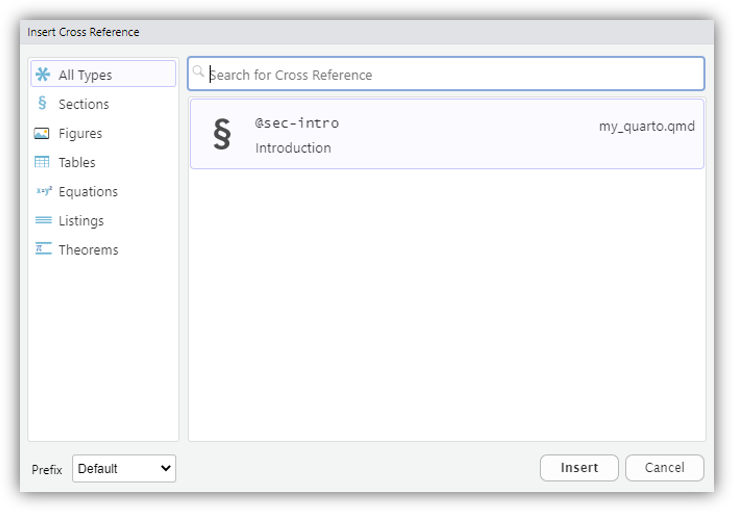
\includegraphics[width=5.5in,height=\textheight]{images/quarto5.png}

}

\end{figure}

\begin{tcolorbox}[enhanced jigsaw, colback=white, toprule=.15mm, arc=.35mm, colbacktitle=quarto-callout-note-color!10!white, titlerule=0mm, colframe=quarto-callout-note-color-frame, title=\textcolor{quarto-callout-note-color}{\faInfo}\hspace{0.5em}{Note}, bottomtitle=1mm, toptitle=1mm, coltitle=black, rightrule=.15mm, opacityback=0, bottomrule=.15mm, breakable, leftrule=.75mm, left=2mm, opacitybacktitle=0.6]

Subsections can be added to a document in a similar fashion using either
\texttt{\#\#} (such that \texttt{\#\#\ Subsection\ \{\#sec-sub\}} will
create a subsection with the label \texttt{sec-sub} and title
\textbf{Subsection}) or by clicking on the
\texttt{Block\ format\ ➠\ Header\ X} menu on the toolbar on the
\texttt{visual} mode.

\end{tcolorbox}

\begin{tcolorbox}[enhanced jigsaw, colback=white, toprule=.15mm, arc=.35mm, colbacktitle=quarto-callout-warning-color!10!white, titlerule=0mm, colframe=quarto-callout-warning-color-frame, title={Task}, bottomtitle=1mm, toptitle=1mm, coltitle=black, rightrule=.15mm, opacityback=0, bottomrule=.15mm, breakable, leftrule=.75mm, left=2mm, opacitybacktitle=0.6]

Try typing \texttt{/} symbol on your main document while using the
visual mode and then use the drop menu to add a new section to your
document ( Tip: you can type the letter \texttt{h} to search for the
different header types while the drop menu is being displayed).

\end{tcolorbox}

\hypertarget{embedding-r-code}{%
\section{Embedding R code}\label{embedding-r-code}}

\hypertarget{code-chunks}{%
\subsection{Code chunks}\label{code-chunks}}

Code chunks allow for R code to be embedded within a document. Not only
can the code be easily included within a document, the code can also be
evaluated. Hence, you can produce an entire report based on an analysis
that is contained within a single file instead of having separate files
containing your R code, plot images and comments.

R Code can be evaluated directly on the Quarto document or in the R
console (the latter would be similar to run your code from an R script).
To select where you want your code to be evaluated click on the setting
options

\includegraphics[width=0.19792in,height=\textheight]{images/settings.png}
(next to the Render button

\includegraphics[width=0.22917in,height=\textheight]{images/rstudio-render-button.png}
) and choose between \texttt{Chunk\ Output\ Inline} (default) if you
want your code to be evaluated within the Quarto document or
\texttt{Chunk\ Output\ in\ Console} to evaluate your code directly on
the R console. If you select the latter, the following options will be
added to the document preamble:

\begin{verbatim}
editor_options: 
  chunk_output_type: inline
\end{verbatim}

To add an R Code Chunk you can simply click on the

\includegraphics[width=0.30208in,height=\textheight]{images/chunk.png}
symbol (or using keyboard shortcut \texttt{cmd+alt+i} or
\texttt{ctrl+alt+i} for windows users) on either \texttt{visual} or
\texttt{source} modes.

R code chunks are identified with~\texttt{\{r\}} with multiple
(optional) chunk options which we can access by typing
\texttt{\#\textbar{}}~at the beginning of the line.

\begin{figure}

{\centering 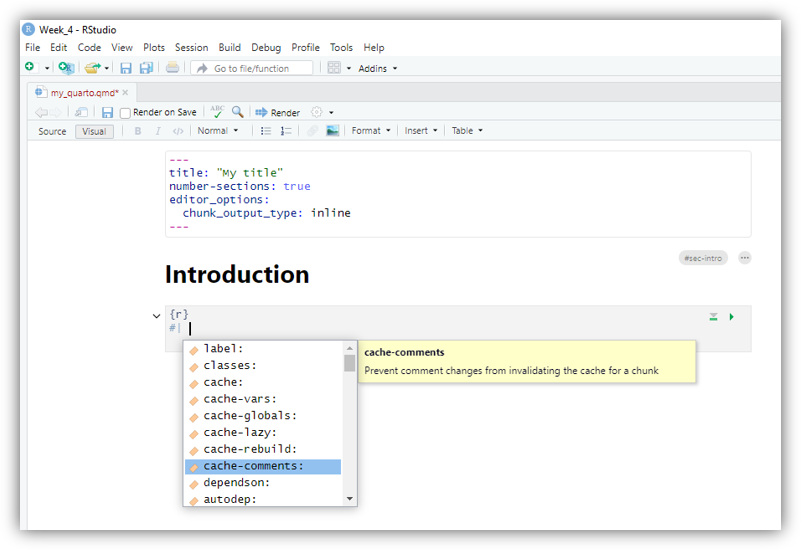
\includegraphics[width=5.05208in,height=\textheight]{images/quarto6.png}

}

\end{figure}

\begin{tcolorbox}[enhanced jigsaw, colback=white, toprule=.15mm, arc=.35mm, colbacktitle=quarto-callout-note-color!10!white, titlerule=0mm, colframe=quarto-callout-note-color-frame, title=\textcolor{quarto-callout-note-color}{\faInfo}\hspace{0.5em}{Note}, bottomtitle=1mm, toptitle=1mm, coltitle=black, rightrule=.15mm, opacityback=0, bottomrule=.15mm, breakable, leftrule=.75mm, left=2mm, opacitybacktitle=0.6]

\hfill\break
If you are in the source mode the R chunks will appear as follow:

\begin{Shaded}
\begin{Highlighting}[]
\InformationTok{\textasciigrave{}\textasciigrave{}\textasciigrave{}\{r\}}

\InformationTok{\textasciigrave{}\textasciigrave{}\textasciigrave{}}
\end{Highlighting}
\end{Shaded}

\end{tcolorbox}

Some of the most common arguments you will use in your R Chunks are:

\begin{itemize}
\tightlist
\item
  \textbf{echo}: include the R code within the code chunk in the
  document (true/false);
\item
  \textbf{eval}: evaluate the R code within the code chunk (true/false);
\item
  \textbf{warning}: suppress warnings from R (true/false); and
\item
  \textbf{message}: suppress messages from R (true/false).
\end{itemize}

For example, let's say we wanted to select the \texttt{score} and
\texttt{bty\_avg} variables from the \texttt{evals} data set to be used
later, we can do that using the following code chunk:

\begin{verbatim}
{r}
#| echo: false
library(tidyverse)
library(moderndive)
evals.scores <- evals |>
  select(score, bty_avg)
\end{verbatim}

Setting \texttt{echo:\ false} will tell the R to evaluate the code while
hiding the R chunk from the main document. In this example, we will
store the subsetted data set as the object \texttt{evals.scores} so that
it can be used later . If you want to embed the code within the Quarto
document then you would simply set \texttt{echo:\ true}.

\begin{tcolorbox}[enhanced jigsaw, colback=white, toprule=.15mm, arc=.35mm, colbacktitle=quarto-callout-important-color!10!white, titlerule=0mm, colframe=quarto-callout-important-color-frame, title=\textcolor{quarto-callout-important-color}{\faExclamation}\hspace{0.5em}{Important}, bottomtitle=1mm, toptitle=1mm, coltitle=black, rightrule=.15mm, opacityback=0, bottomrule=.15mm, breakable, leftrule=.75mm, left=2mm, opacitybacktitle=0.6]

R chunk options are case sensitive! so \texttt{echo:\ TRUE} or
\texttt{echo:\ FALSE} won't work! You can use R Studio autocomplete
feature the see the available options by pressing the tab key.

\end{tcolorbox}

Note that by default Quarto will set \texttt{echo:\ true} .
Alternatively, you can edit the Quarto preamble and change the global
output options to show or hide all R chunks. You can do this within the
\texttt{execute} options as follows (you can manually override this by
changing the \texttt{echo} option in each individual chunk) :

\begin{verbatim}
---
title: "My title"
number-sections: true
execute:
  echo: false
---
\end{verbatim}

\begin{tcolorbox}[enhanced jigsaw, colback=white, toprule=.15mm, arc=.35mm, colbacktitle=quarto-callout-important-color!10!white, titlerule=0mm, colframe=quarto-callout-important-color-frame, title=\textcolor{quarto-callout-important-color}{\faExclamation}\hspace{0.5em}{Important}, bottomtitle=1mm, toptitle=1mm, coltitle=black, rightrule=.15mm, opacityback=0, bottomrule=.15mm, breakable, leftrule=.75mm, left=2mm, opacitybacktitle=0.6]

You need to be very careful with the indentation if you decide to change
the global settings of Quarto preamble!

\end{tcolorbox}

Lets look at another example:

\begin{Shaded}
\begin{Highlighting}[]
\InformationTok{\textasciigrave{}\textasciigrave{}\textasciigrave{}\{r\}}
\CommentTok{\#| message: false}
\CommentTok{\#| warning: false}
\FunctionTok{library}\NormalTok{(gapminder)}
\FunctionTok{library}\NormalTok{(skimr)}
\FunctionTok{library}\NormalTok{(ggplot2)}
\InformationTok{\textasciigrave{}\textasciigrave{}\textasciigrave{}}
\end{Highlighting}
\end{Shaded}

In this case, we set \texttt{warning} and \texttt{message} to
\texttt{false} to indicate that we want to suppress any warnings or
messages (e.g., the ones that you usually get when loading R packages).
Another useful options is \texttt{eval.} If we set \texttt{eval:\ false}
then we indicate that we don't want the chunk output to be included in
the rendered document (this is useful for example if we just want to
show our R code without rendering its output):

\begin{Shaded}
\begin{Highlighting}[]
\InformationTok{\textasciigrave{}\textasciigrave{}\textasciigrave{}\{r\}}
\CommentTok{\#| eval: false}

\FunctionTok{ggplot}\NormalTok{(}\AttributeTok{data=}\NormalTok{evals.scores,}\FunctionTok{aes}\NormalTok{(}\AttributeTok{y=}\NormalTok{score,}\AttributeTok{x=}\NormalTok{bty\_avg)) }\SpecialCharTok{+}
  \FunctionTok{geom\_point}\NormalTok{()}
\InformationTok{\textasciigrave{}\textasciigrave{}\textasciigrave{}}
\end{Highlighting}
\end{Shaded}

\begin{tcolorbox}[enhanced jigsaw, colback=white, toprule=.15mm, arc=.35mm, colbacktitle=quarto-callout-note-color!10!white, titlerule=0mm, colframe=quarto-callout-note-color-frame, title=\textcolor{quarto-callout-note-color}{\faInfo}\hspace{0.5em}{Note}, bottomtitle=1mm, toptitle=1mm, coltitle=black, rightrule=.15mm, opacityback=0, bottomrule=.15mm, breakable, leftrule=.75mm, left=2mm, opacitybacktitle=0.6]

Note that we can still run the code in each individual chunk (even if we
set \texttt{eval:\ false}) by clicking the run chunk
bottom
\includegraphics[width=0.29167in,height=0.1875in]{images/run_chunk.png}.
The code will be evaluated in either your \texttt{.qmd} file or in the
console depending on the Chunk output settings (this mean that can test
your code in R but its output won;t be rendered in the final dicument).

\end{tcolorbox}

Additional arguments can be passed to code chunks other than those
displayed above. The most useful ones other than those relate to figure
sizing and positioning and are discussed in the upcoming sections.

\hypertarget{inline-code}{%
\subsection{Inline code}\label{inline-code}}

R code can be included within text by enclosing the code with
\texttt{\textasciigrave{}r\ \textasciigrave{}}. This allows for
expressions to be evaluated by R and not be hardwired by the user. For
example, if you wanted to convey the number of observations within
\texttt{evals.scores} then we can enclose \texttt{nrow(evals.scores)}
within \texttt{\textasciigrave{}r\ \textasciigrave{}} to obtain the
number of observations, rather than hardwiring 463 into the text. This
can help to prevent potential human error when presenting information.
It can also help with consistency and ease-of-use, since
\texttt{n\ =\ nrow(evals.scores)} could be stored as an R object and
referred to whenever necessary within the text using inline R code.

\hypertarget{tables}{%
\section{Tables}\label{tables}}

There are several ways to produce tables in Quarto . Here, a couple of
different approaches will be presented. The first approach uses the
\texttt{gt()} function from the \texttt{gt} package and essentially puts
a wrapper around the tables produced in R in order to make them more
visually appealing within the Quarto document. Here we will just cover
the basics, but if you want to learn more about creating eye-catching
tables with \texttt{gt} visit
\href{https://gt.rstudio.com/articles/intro-creating-gt-tables.html}{here}.

Let's say we wanted to create a table of the first 5 rows of the
\texttt{iris} data from the \texttt{datasets} library. We can create the
table using the \texttt{gt} function as follows:

\begin{Shaded}
\begin{Highlighting}[]
\FunctionTok{library}\NormalTok{(gt)}

\NormalTok{iris }\SpecialCharTok{|\textgreater{}} 
  \FunctionTok{slice\_head}\NormalTok{(}\AttributeTok{n=}\DecValTok{5}\NormalTok{) }\SpecialCharTok{|\textgreater{}}
  \FunctionTok{gt}\NormalTok{() }
\end{Highlighting}
\end{Shaded}

\begin{longtable*}{rrrrc}
\toprule
Sepal.Length & Sepal.Width & Petal.Length & Petal.Width & Species \\ 
\midrule\addlinespace[2.5pt]
5.1 & 3.5 & 1.4 & 0.2 & setosa \\ 
4.9 & 3.0 & 1.4 & 0.2 & setosa \\ 
4.7 & 3.2 & 1.3 & 0.2 & setosa \\ 
4.6 & 3.1 & 1.5 & 0.2 & setosa \\ 
5.0 & 3.6 & 1.4 & 0.2 & setosa \\ 
\bottomrule
\end{longtable*}

Lets customize this table a bit by (1) adding a table caption and number
(2) modifying the labels of the columns and (3) create a grouping
structure for the petals and sepals width and length columns:

\begin{Shaded}
\begin{Highlighting}[]
\InformationTok{\textasciigrave{}\textasciigrave{}\textasciigrave{}\{r\}}
\CommentTok{\#| label: tbl{-}iris}
\CommentTok{\#| tbl{-}cap: First five entries of the iris Data set}

\NormalTok{iris }\SpecialCharTok{|\textgreater{}} 
  \FunctionTok{slice\_head}\NormalTok{(}\AttributeTok{n=}\DecValTok{5}\NormalTok{) }\SpecialCharTok{|\textgreater{}}
  \FunctionTok{gt}\NormalTok{() }\SpecialCharTok{|\textgreater{}}
   \FunctionTok{fmt\_number}\NormalTok{(}\AttributeTok{decimals=}\DecValTok{2}\NormalTok{) }\SpecialCharTok{|\textgreater{}}
 \FunctionTok{tab\_spanner}\NormalTok{(}
    \AttributeTok{label =} \StringTok{"Sepals"}\NormalTok{,}
    \AttributeTok{columns =} \FunctionTok{c}\NormalTok{(Sepal.Length, Sepal.Width)}
\NormalTok{  ) }\SpecialCharTok{|\textgreater{}}
  \FunctionTok{tab\_spanner}\NormalTok{(}
    \AttributeTok{label =} \StringTok{"Petals"}\NormalTok{,}
    \AttributeTok{columns =} \FunctionTok{c}\NormalTok{(Petal.Length, Petal.Width)}
\NormalTok{  ) }\SpecialCharTok{|\textgreater{}}
  \FunctionTok{cols\_label}\NormalTok{(}
    \AttributeTok{Sepal.Length =} \FunctionTok{html}\NormalTok{(}\StringTok{"Length (cm)"}\NormalTok{),}
    \AttributeTok{Sepal.Width =} \FunctionTok{html}\NormalTok{(}\StringTok{"Width (cm)"}\NormalTok{),}
    \AttributeTok{Petal.Length =} \FunctionTok{html}\NormalTok{(}\StringTok{"Length (cm)"}\NormalTok{),}
    \AttributeTok{Petal.Width =} \FunctionTok{html}\NormalTok{(}\StringTok{"Width (cm)"}\NormalTok{)}
\NormalTok{  )}
\InformationTok{\textasciigrave{}\textasciigrave{}\textasciigrave{}}
\end{Highlighting}
\end{Shaded}

\hypertarget{tbl-iris}{}
\begin{longtable}{rrrrc}
\caption{\label{tbl-iris}First five entries of the iris Data set }\tabularnewline

\toprule
\multicolumn{2}{c}{Sepals} & \multicolumn{2}{c}{Petals} &  \\ 
\cmidrule(lr){1-2} \cmidrule(lr){3-4}
Length (cm) & Width (cm) & Length (cm) & Width (cm) & Species \\ 
\midrule\addlinespace[2.5pt]
$5.10$ & $3.50$ & $1.40$ & $0.20$ & setosa \\ 
$4.90$ & $3.00$ & $1.40$ & $0.20$ & setosa \\ 
$4.70$ & $3.20$ & $1.30$ & $0.20$ & setosa \\ 
$4.60$ & $3.10$ & $1.50$ & $0.20$ & setosa \\ 
$5.00$ & $3.60$ & $1.40$ & $0.20$ & setosa \\ 
\bottomrule
\end{longtable}

The first thing we've done is to add a table label using
\texttt{label:\ tbl-planets} .This will allow us to add cross-reference
in the text (Remember to use the \texttt{tbl-}~prefix to make them
cross-referenceable). For example we can write \texttt{@tbl-iris} in our
document to reference and create an hyperlink directed to the
Table~\ref{tbl-iris} (you can also use the tool bar
\texttt{Insert▾➠\ Cross\ Reference} to do this). Then, the option
\texttt{tbl-cap:} allow us to add caption to the table. Finally, we set
the number of decimals to 2 with the \texttt{fmt\_number} function and
then we use the \texttt{tab\_spanner} and \texttt{cols\_label} functions
to change some features of our \texttt{gt} table.

\hypertarget{tables-by-hand}{%
\subsection{Tables `by hand'}\label{tables-by-hand}}

Tables can also be produced `by hand' in Quarto . For example, the table
above corresponding to the first 5 rows of the \texttt{iris} data can be
produced by hand by clicking on the \texttt{Table} option in the toolbar
(next to \texttt{Insert▾} while using the \texttt{visual} mode) and
selecting the number of rows and columns.

\begin{figure}

{\centering 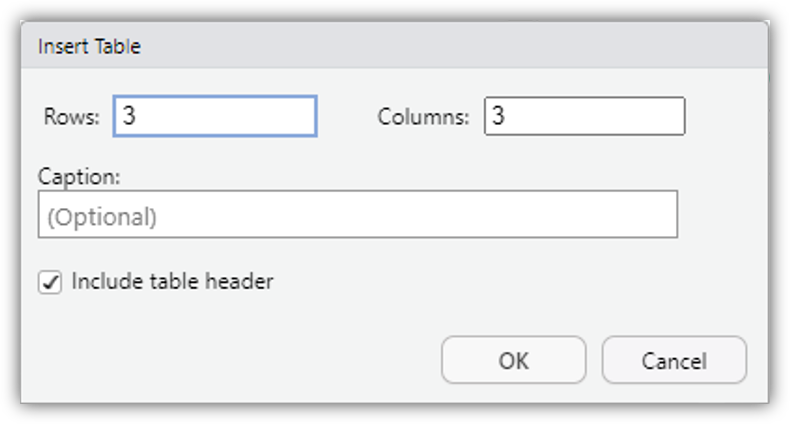
\includegraphics[width=4.53125in,height=\textheight]{images/quarto7.png}

}

\end{figure}

We can manually fill each entry to produce the following table:

\begin{longtable}[]{@{}ccccr@{}}
\caption{The fist 5 rows of the iris data.}\tabularnewline
\toprule\noalign{}
Sepal Length & Sepal Width & Petal Length & Petal Width & Species \\
\midrule\noalign{}
\endfirsthead
\toprule\noalign{}
Sepal Length & Sepal Width & Petal Length & Petal Width & Species \\
\midrule\noalign{}
\endhead
\bottomrule\noalign{}
\endlastfoot
5.1 & 3.5 & 1.4 & 0.2 & setosa \\
4.9 & 3.0 & 1.4 & 0.2 & setosa \\
4.7 & 3.2 & 1.3 & 0.2 & setosa \\
4.6 & 3.1 & 1.5 & 0.2 & setosa \\
5.0 & 3.6 & 1.4 & 0.2 & setosa \\
\end{longtable}

If you then go to the \texttt{source} mode you will see the raw markdown
code that produced this table:

\begin{verbatim}
| Sepal Length | Sepal Width | Petal Length | Petal Width | Species |
|:------------:|:-----------:|:------------:|:-----------:|--------:|
|     5.1      |     3.5     |     1.4      |     0.2     |  setosa |
|     4.9      |     3.0     |     1.4      |     0.2     |  setosa |
|     4.7      |     3.2     |     1.3      |     0.2     |  setosa |
|     4.6      |     3.1     |     1.5      |     0.2     |  setosa |
|     5.0      |     3.6     |     1.4      |     0.2     |  setosa |
: The fist 5 rows of the iris data. {#tbl-iris}
\end{verbatim}

In here, the vertical separators \texttt{\textbar{}} are used between
columns, while \texttt{-\/-\/-} is placed below table/column headings.
Alignment of the columns is done using colons, that is, for left
alignment put \texttt{:-\/-\/-}, for right alignment put
\texttt{-\/-\/-:}, and for centred alignment put \texttt{:-\/-\/-:}. For
these sorts of tables, you can add a caption below the table and then
include a \texttt{\#tbl-\ label} in braces at the end of the caption for
cross-referencing.

\begin{tcolorbox}[enhanced jigsaw, colback=white, toprule=.15mm, arc=.35mm, colbacktitle=quarto-callout-note-color!10!white, titlerule=0mm, colframe=quarto-callout-note-color-frame, title=\textcolor{quarto-callout-note-color}{\faInfo}\hspace{0.5em}{Note}, bottomtitle=1mm, toptitle=1mm, coltitle=black, rightrule=.15mm, opacityback=0, bottomrule=.15mm, breakable, leftrule=.75mm, left=2mm, opacitybacktitle=0.6]

You can read more about authoring Quarto tables
\href{https://quarto.org/docs/authoring/tables.html}{here}.

\end{tcolorbox}

\hypertarget{figures}{%
\section{Figures}\label{figures}}

\hypertarget{embedding-external-images}{%
\subsection{Embedding external images}\label{embedding-external-images}}

Including plots and figures within a Quarto document is straightforward.
To include an external figure you can use the \texttt{visual} mode tool
bar and click on \texttt{Insert▾➠\ Figure/Image...} and then browse to
the path where you image is, or alternatively write the \emph{url} from
which the image should be obtained. The pop-up windows allows you also
to write a caption and also to modify the image alignment with respect
the main text.

\begin{figure}

{\centering 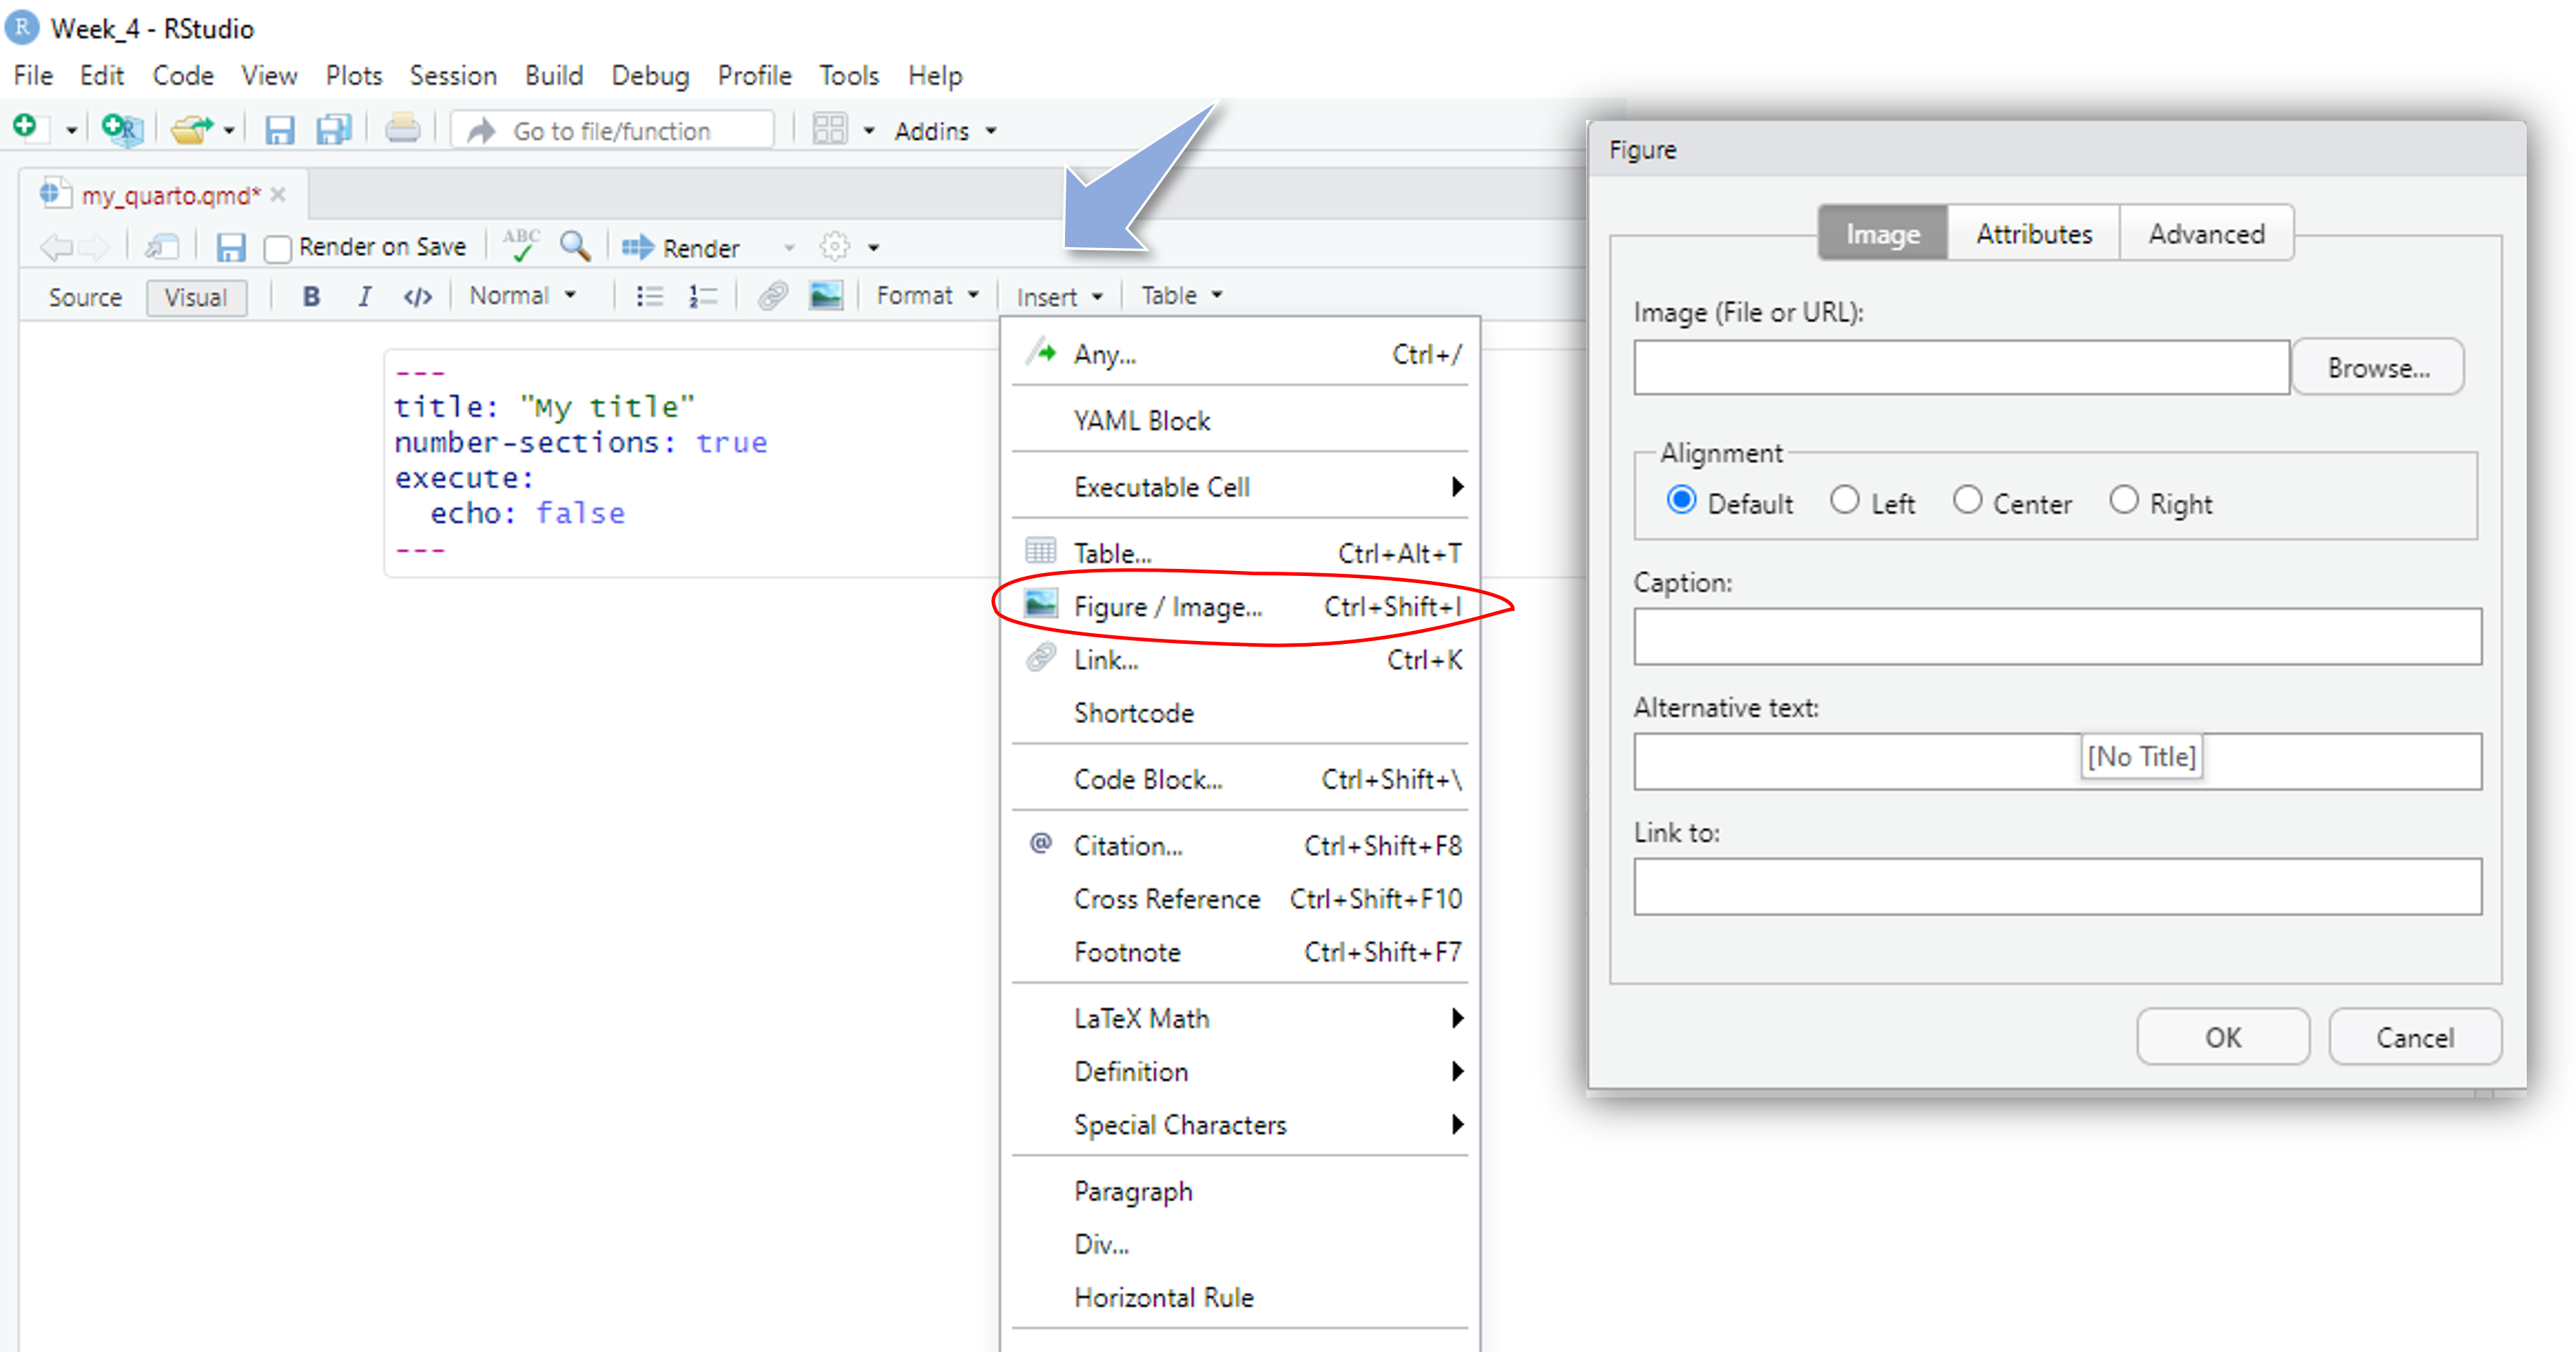
\includegraphics{images/quarto8.png}

}

\end{figure}

If you want to add cross-referencing you can add the \texttt{fig-}
prefix in the attributes tab of the pop-up windows:

\begin{figure}

{\centering 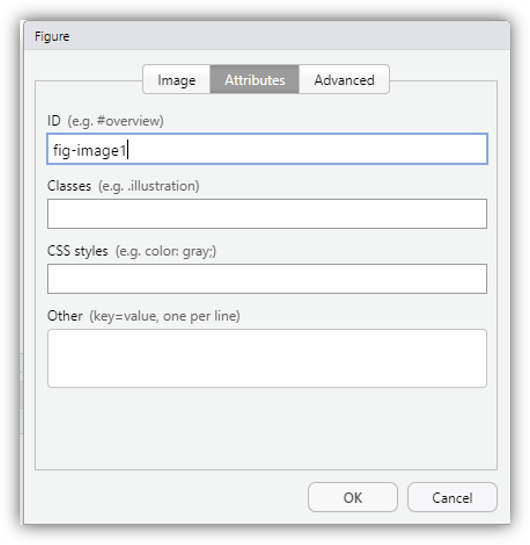
\includegraphics[width=3.94792in,height=\textheight]{images/quarto9.png}

}

\end{figure}

The source code would then look something like:

\begin{verbatim}
![](images/myimage.png){#fig-image1}
\end{verbatim}

\hypertarget{embedding-r-generated-figures}{%
\subsection{Embedding R generated
figures}\label{embedding-r-generated-figures}}

Very often we would like to use the R plots generated from your analysis
instead of using external figures. To achieve this, the R code for the
plot is simply included within a code chunk including additional
arguments for plot size and positioning. For example, to include the
scatterplot of teaching and beauty:

\begin{Shaded}
\begin{Highlighting}[]
\InformationTok{\textasciigrave{}\textasciigrave{}\textasciigrave{}\{r\}}
\CommentTok{\#| label: fig{-}scatterplot1}
\CommentTok{\#| fig{-}cap: Relationship between teaching and beauty scores. The best{-}fitting line has been superimposed.}
\CommentTok{\#| fig{-}width: 4}
\CommentTok{\#| fig{-}height: 5}
\CommentTok{\#| fig{-}align: center}
\CommentTok{\#| message: false}

\FunctionTok{ggplot}\NormalTok{(evals.scores, }\FunctionTok{aes}\NormalTok{(}\AttributeTok{x =}\NormalTok{ bty\_avg, }\AttributeTok{y =}\NormalTok{ score)) }\SpecialCharTok{+}
  \FunctionTok{geom\_point}\NormalTok{() }\SpecialCharTok{+}
  \FunctionTok{labs}\NormalTok{(}\AttributeTok{x =} \StringTok{"Beauty Score"}\NormalTok{, }\AttributeTok{y =} \StringTok{"Teaching Score"}\NormalTok{) }\SpecialCharTok{+}
  \FunctionTok{geom\_smooth}\NormalTok{(}\AttributeTok{method =} \StringTok{"lm"}\NormalTok{, }\AttributeTok{se =} \ConstantTok{FALSE}\NormalTok{)}
\InformationTok{\textasciigrave{}\textasciigrave{}\textasciigrave{}}
\end{Highlighting}
\end{Shaded}

\begin{figure}[H]

{\centering 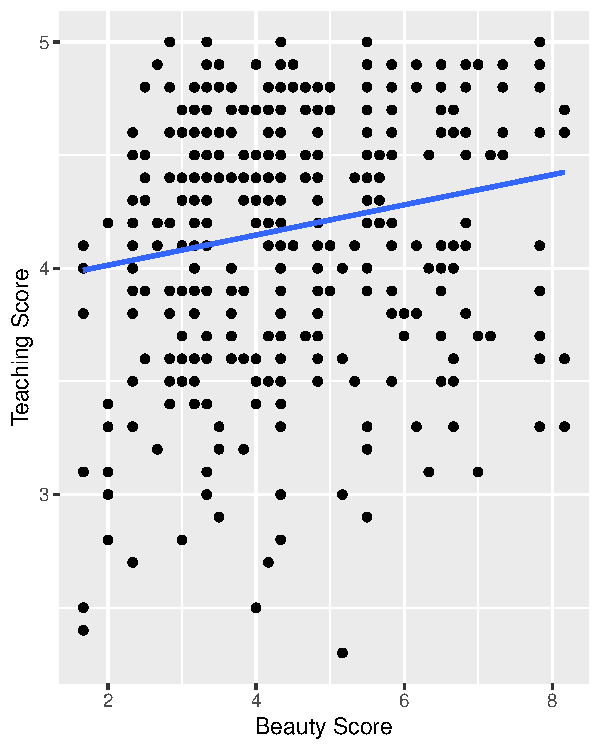
\includegraphics{index_files/figure-pdf/fig-scatterplot1-1.pdf}

}

\caption{\label{fig-scatterplot1}Relationship between teaching and
beauty scores. The best-fitting line has been superimposed.}

\end{figure}

Here, we set the chunk label to include the \texttt{fig-} prefix so we
can cross-reference using the @ prefix. For example
\texttt{@fig-scatterplot1} will create a hyperlink to
Figure~\ref{fig-scatterplot1}. Then we added a figure caption using the
\texttt{fig-cap} option. For size and positioning of the figure we can
include:

\begin{itemize}
\tightlist
\item
  \texttt{fig.width}: an integer value denoting the width of the figure;
\item
  \texttt{fig.height}: an integer value denoting the height of the
  figure;
\item
  \texttt{fig.align}: the alignment of the figure within the body of the
  document
\end{itemize}

\begin{tcolorbox}[enhanced jigsaw, colback=white, toprule=.15mm, arc=.35mm, colbacktitle=quarto-callout-tip-color!10!white, titlerule=0mm, colframe=quarto-callout-tip-color-frame, title={Question}, bottomtitle=1mm, toptitle=1mm, coltitle=black, rightrule=.15mm, opacityback=0, bottomrule=.15mm, breakable, leftrule=.75mm, left=2mm, opacitybacktitle=0.6]

What other argument would you need to include if you wish to show the
chunk plot output only?

\begin{itemize}
\item
  \begin{enumerate}
  \def\labelenumi{(\Alph{enumi})}
  \tightlist
  \item
    eval: false\\
  \end{enumerate}
\item
  \begin{enumerate}
  \def\labelenumi{(\Alph{enumi})}
  \setcounter{enumi}{1}
  \tightlist
  \item
    echo: true\\
  \end{enumerate}
\item
  \begin{enumerate}
  \def\labelenumi{(\Alph{enumi})}
  \setcounter{enumi}{2}
  \tightlist
  \item
    echo: false\\
  \end{enumerate}
\item
  \begin{enumerate}
  \def\labelenumi{(\Alph{enumi})}
  \setcounter{enumi}{3}
  \tightlist
  \item
    eval: true
  \end{enumerate}
\end{itemize}

\end{tcolorbox}

\begin{tcolorbox}[enhanced jigsaw, colback=white, toprule=.15mm, arc=.35mm, colbacktitle=quarto-callout-note-color!10!white, titlerule=0mm, colframe=quarto-callout-note-color-frame, title=\textcolor{quarto-callout-note-color}{\faInfo}\hspace{0.5em}{Note}, bottomtitle=1mm, toptitle=1mm, coltitle=black, rightrule=.15mm, opacityback=0, bottomrule=.15mm, breakable, leftrule=.75mm, left=2mm, opacitybacktitle=0.6]

You can read more about authoring Quarto tables
\href{https://quarto.org/docs/authoring/figures.html}{here}.

\end{tcolorbox}

\hypertarget{mathematics}{%
\section{Mathematics}\label{mathematics}}

Mathematics and statistical equations can be presented nicely within a
Quarto document. For example, the following equation referring to a
linear regression model:

\[y_i = \alpha + \beta x_i + \epsilon_i, ~~~~ \epsilon_i \sim N(0, \sigma^2),\]
is done using the following:

\texttt{\$\$\ y\_i\ =\ \textbackslash{}alpha\ +\ \textbackslash{}beta\ x\_i\ +\ \textbackslash{}epsilon\_i,\ \textasciitilde{}\textasciitilde{}\textasciitilde{}\textasciitilde{}\textasciitilde{}\ \textbackslash{}\textasciigrave{}\textasciigrave{}epsilon\_i\textasciigrave{}\textasciigrave{}\textbackslash{}sim\ N(0,\ \textbackslash{}sigma\^{}2),\ \$\$}

That is, we use:

\begin{itemize}
\tightlist
\item
  \texttt{\$\$} signs to produce mathematics which is centred, and a
  single \texttt{\$} to include mathematics within a sentence or
  paragraph; in visual mode you can go to
  \texttt{Insert\ ▾\ \ ➠\ LaTeX\ Math\ ▸} and chose between
  \texttt{Inlay\ Math} or \texttt{Display\ Math}.
\item
  \texttt{\_} and \texttt{\^{}} are used for subscripts and
  superscripts, respectively;
\item
  Greek letters are obtained using \texttt{\textbackslash{}} and the
  letters name, i.e.~\texttt{\textbackslash{}alpha} gives \(\alpha\);
  and
\item
  tildes (\texttt{\textasciitilde{}}) are used to put spacing between
  notation.
\end{itemize}

If you have a categorical variable then you would write it using an
indicator function. For example, if we have gender as a categorical
variable, where females are the baseline category, then we could write
our model as follows:

\[y_i = \alpha + \beta_{\mbox{Male}} \cdot \mathbb{I}_{\mbox{Male}}(x),\]

\begin{verbatim}
$$y_i = \alpha + \beta_{\mbox{Male}} \cdot \mathbb{I}_{\mbox{Male}}(x),$$
\end{verbatim}

where \(\mathbb{I}_{\mbox{Male}}(x)\)
\texttt{\$\textbackslash{}mathbb\{I\}\_\{\textbackslash{}mbox\{Male\}\}(x)\$}
is an indicator function such that

\[\mathbb{I}_{\mbox{Male}}(x)=\left\{
                \begin{array}{ll}
                  1 ~~~ \mbox{if the gender of} ~ x \mbox{th observation is Male},\\
                  0 ~~~ \mbox{Otherwise}.\\
                \end{array}
              \right.\]

\begin{verbatim}
    $$\mathbb{I}_{\mbox{Male}}(x)=\left\{
                \begin{array}{ll}
                  1 ~~~ \mbox{if Gender of} ~ x \mbox{th observation is Male},\\
                  0 ~~~ \mbox{Otherwise}.\\
                \end{array}
              \right.$$
\end{verbatim}

\begin{tcolorbox}[enhanced jigsaw, colback=white, toprule=.15mm, arc=.35mm, colbacktitle=quarto-callout-note-color!10!white, titlerule=0mm, colframe=quarto-callout-note-color-frame, title=\textcolor{quarto-callout-note-color}{\faInfo}\hspace{0.5em}{Note}, bottomtitle=1mm, toptitle=1mm, coltitle=black, rightrule=.15mm, opacityback=0, bottomrule=.15mm, breakable, leftrule=.75mm, left=2mm, opacitybacktitle=0.6]

For additional tricks inserting mathematics into documents see
\href{https://quarto.org/docs/visual-editor/technical.html}{here}.

\end{tcolorbox}

\hypertarget{quarto-presentations}{%
\section{Quarto Presentations}\label{quarto-presentations}}

Another great feature of Quarto is that it allows you to create
presentations and supports a variety of formats such as
\href{https://quarto.org/docs/presentations/revealjs/}{html},
\href{https://quarto.org/docs/presentations/powerpoint.html}{power
point} and
\href{https://quarto.org/docs/presentations/beamer.html}{beamer}. Today
we will focus on creating an html presentation (which can be also
printed as a pdf).

Creating an html presentation is as easy as setting the output format to
\texttt{revealjs}:

\begin{verbatim}



---
title: "My title"
author: "Jafet Belmont"
format: revealjs
---


\end{verbatim}

This will create a title slide that includes the provided \texttt{title}
and \texttt{author}. (you can remove any of these options if you the
author or title page to be removed). Now we will switch to the
\texttt{visual} mode. You will notice that a new set of options have now
appeared:

\begin{figure}

{\centering 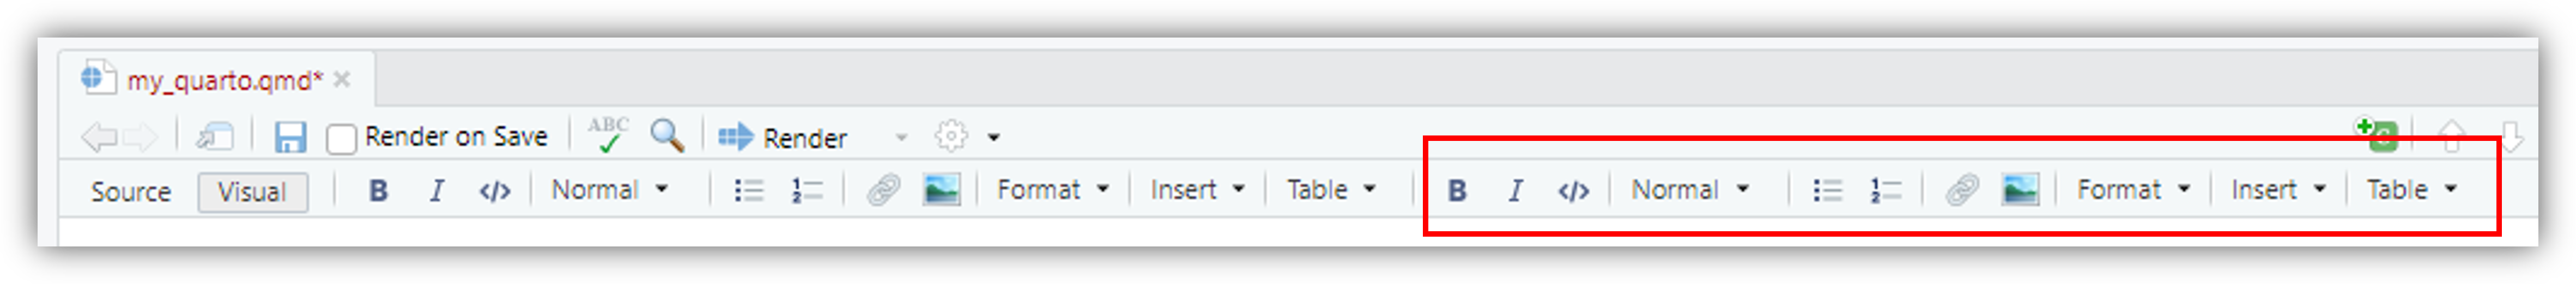
\includegraphics{images/quarto13.png}

}

\end{figure}

This new tab will allow us to interact with the different features of
our presentation. Lets begin by creating some slides. Slides in Quarto
are delineated using level 1 and 2 headings:

\begin{verbatim}



---
title: "My title"
author: "Jafet Belmont"
format: revealjs
---




# Topic 1


## Slide 1.1


# Topic 2


## Slide 2.1
\end{verbatim}

In the example above we use level 1 headings for creating a new sections
and level 2 heading for defining the new slides. Alternatively we can
use horizontal rules to create the slides as follows (on \texttt{visual}
mode click on \texttt{Insert▾\ ➠\ Horizontal\ Rule}):

\begin{verbatim}



---
title: "My title"
author: "Jafet Belmont"
format: revealjs
---




  Content of slide 1

---

  Content of slide 2




---
\end{verbatim}

You can add bullet and numbered lists to each slide as follows (on
\texttt{visual} mode click on

\includegraphics[width=0.25in,height=0.26042in]{images/bullets.png} or

\includegraphics[width=0.3125in,height=0.26042in]{images/numbered.png}
for adding bullet or numbered lists respectively):

\begin{verbatim}
---



title: "My title"
author: "Jafet Belmont"
format: revealjs

---

## Slide 1

1.  Item 1
2.  Item 2

## Slide 2

-   Bullet 1

    -   Bullet 1.1

    -   Bullet 1.2

-   Bulet 2

    -   Bullet 2.1

    -   Bullet 2.2
\end{verbatim}

Notice that indentation allow us to create a hierarchical structure
within our lists of items. You can modify some of the option of the list
by clicking the

\includegraphics[width=0.15625in,height=\textheight]{images/threedots.png}
button on the right side of it. This will open a pop-up window where you
can modify some of its attributes. For example, you can ask Quarto to
display each item one by one as you move forward through the slides:

\begin{figure}

{\centering 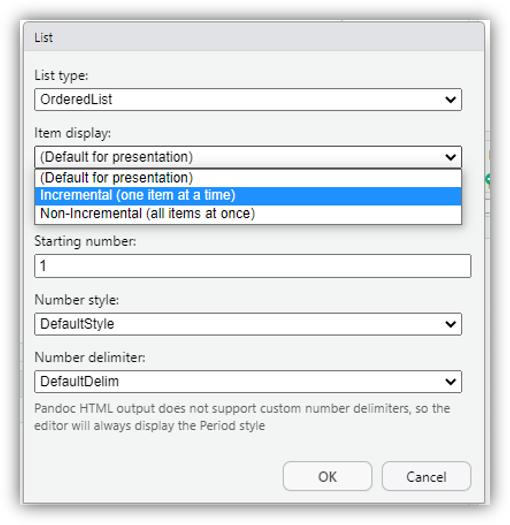
\includegraphics[width=3.8125in,height=\textheight]{images/quarto11.png}

}

\end{figure}

If you want to arrange the content of you slide into different columns
you can insert a multiple column output. To do this switch to
\texttt{visual} mode and click on \texttt{Insert▾\ ➠\ Slide\ Columns}).
You can then fill each column:

\begin{figure}

{\centering 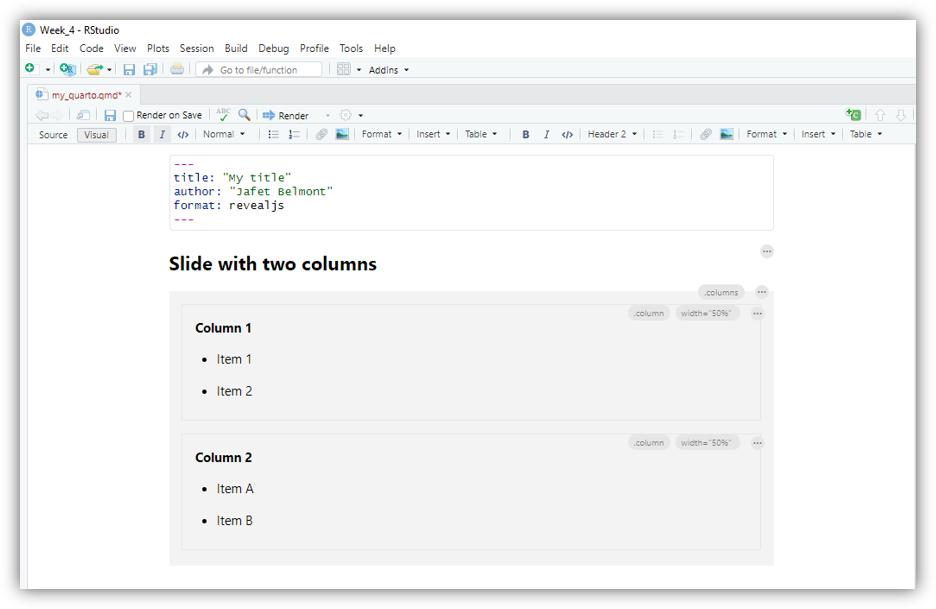
\includegraphics{images/quarto12.png}

}

\end{figure}

Sometimes the text size in your slide might be too large to fit in your
slide and you would like to make it smaller. You can then use the
.smaller class to use a smaller typeface so that more text fits on the
slide.

\begin{verbatim}

---

title: "My title"
author: "Jafet Belmont"
format: revealjs

---


## Slide with small text {.smaller}

1.  Item 1
2.  Item 2
 
\end{verbatim}

~If you are on the visual model, click on the slide settings

\includegraphics[width=0.17708in,height=\textheight]{images/threedots.png}
and then type \texttt{.smaller} on the class box:

\begin{figure}

{\centering 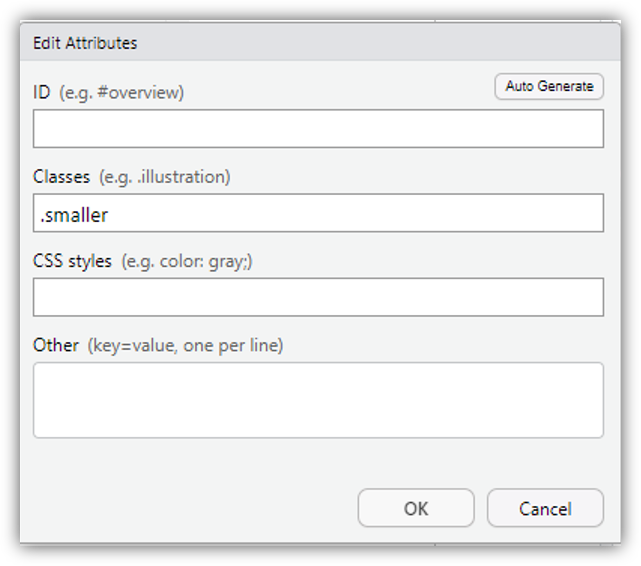
\includegraphics[width=3.88542in,height=\textheight]{images/quarto14.png}

}

\end{figure}

\begin{tcolorbox}[enhanced jigsaw, colback=white, toprule=.15mm, arc=.35mm, colbacktitle=quarto-callout-note-color!10!white, titlerule=0mm, colframe=quarto-callout-note-color-frame, title=\textcolor{quarto-callout-note-color}{\faInfo}\hspace{0.5em}{Note}, bottomtitle=1mm, toptitle=1mm, coltitle=black, rightrule=.15mm, opacityback=0, bottomrule=.15mm, breakable, leftrule=.75mm, left=2mm, opacitybacktitle=0.6]

Note that ideally you slides should not contain too much text and thus
this is just a quick way around if you feel that you need a bit of extra
space in your slide.

\end{tcolorbox}

R code can be embedded in any slides by including a R chunk in the same
way as we did before. However, sometimes we would like to arrange the
code output to be display in a ``tidy'' manner within the slide. To
achieve this we can use the \texttt{output-location:} argument which has
the following options:

\begin{itemize}
\item
  \texttt{column}: Display output in a column adjacent to the code
\item
  \texttt{column-fragment}: Display output in a column adjacent to the
  code and delay showing it until its explicitly stepped through by
  advancing the slides.
\item
  \texttt{fragment}: Delay the output dipslay until it is explicitly
  stepped through by advancing the slides.
\item
  \texttt{slide}: Display output on the subsequent slide.

  For example, the source code for a slide containing an R code would
  look something like this:

\begin{verbatim}
---
title: "My title"
author: "Jafet Belmont"
format: revealjs
---

## Slide with R Code {.smaller}

::: {.cell output-location='column-fragment'}

```{.r .cell-code}
ggplot(evals.scores, aes(x = bty_avg, y = score)) +
  geom_point() +
  labs(x = "Beauty Score", y = "Teaching Score") +
  geom_smooth(method = "lm", se = FALSE)
```

::: {.cell-output .cell-output-stderr}
```
`geom_smooth()` using formula = 'y ~ x'
```
:::

::: {.cell-output-display}
![](index_files/figure-pdf/unnamed-chunk-8-1.pdf){fig-pos='H'}
:::
:::
\end{verbatim}
\end{itemize}

\hypertarget{rendering}{%
\section{Rendering}\label{rendering}}

You can render a Quarto document or a presentation by clicking the
Render button

\includegraphics[width=0.22917in,height=\textheight]{images/rstudio-render-button.png}.

\begin{tcolorbox}[enhanced jigsaw, colback=white, toprule=.15mm, arc=.35mm, colbacktitle=quarto-callout-note-color!10!white, titlerule=0mm, colframe=quarto-callout-note-color-frame, title=\textcolor{quarto-callout-note-color}{\faInfo}\hspace{0.5em}{Note}, bottomtitle=1mm, toptitle=1mm, coltitle=black, rightrule=.15mm, opacityback=0, bottomrule=.15mm, breakable, leftrule=.75mm, left=2mm, opacitybacktitle=0.6]

Note that if you are working on a Quarto document you can also compile a
PDF version of it by clicking on

\includegraphics[width=0.17708in,height=0.17708in]{images/rstudio-render-button.png}\texttt{Render\ ▾\ ➠}
\includegraphics[width=0.14583in,height=\textheight]{images/renderpdf.png}\texttt{Render\ PDF}.
However, if you are working on a Quarto presentation while using
\texttt{revealjs} format then you need to render the presentation first
in html and then export it as pdf by following these
\href{https://quarto.org/docs/presentations/revealjs/presenting.html\#print-to-pdf}{instructions}.

\end{tcolorbox}

When you render a Quarto document, the R code in you chunks is executed
by the \href{http://yihui.name/knitr/}{knitr}~R-package and a new
markdown (.md) document is then created. This file includes all of your
code and its output. \href{http://pandoc.org/}{pandoc} then processes
this markdown to create the finished format. \emph{The Render button
encapsulates these actions and executes them in the right order for
you.}

\begin{figure}

{\centering 
\includegraphics{images/rstudio-qmd-how-it-works.png}

}

\end{figure}

Note that HTML rendered documents will typically have a number of
external dependencies (e.g.~images, CSS style sheets, JavaScript, etc.)
which are contained in an external \texttt{\_files} directory alongside
your document. If you share youe HTML rendered file without the external
files, it will lose all of its previous formatting and style.
Alternatively, you can create a self-contained HTML document using the
the \texttt{embed-resources} option in quarto as follows:

\begin{verbatim}

---

title: "My document"
format:
  html:
    embed-resources: true

---
\end{verbatim}

This will create standalone HTML file with no external dependencies that
you can share with others (note that indentation here is important as
you are calling arguments within the format output) .

\begin{tcolorbox}[enhanced jigsaw, colback=white, toprule=.15mm, arc=.35mm, colbacktitle=quarto-callout-important-color!10!white, titlerule=0mm, colframe=quarto-callout-important-color-frame, title=\textcolor{quarto-callout-important-color}{\faExclamation}\hspace{0.5em}{Important}, bottomtitle=1mm, toptitle=1mm, coltitle=black, rightrule=.15mm, opacityback=0, bottomrule=.15mm, breakable, leftrule=.75mm, left=2mm, opacitybacktitle=0.6]

For your upcoming class test you want to make sure this option is set to
\texttt{true} so your work can be displayed properly by a browser.

\end{tcolorbox}



\end{document}
